\documentclass[11pt,a4paper,fontset=windows]{ctexart}

\usepackage{geometry}
\geometry{left=2.6cm,right=2.6cm,top=2.6cm,bottom=2.6cm}
\usepackage{graphicx}
\usepackage{booktabs}
\usepackage{amsmath}
\usepackage{amssymb}
\usepackage{xcolor}
\usepackage{tikz}
\usetikzlibrary{arrows.meta,positioning}
\usepackage{natbib}
\usepackage{url}
\usepackage[hidelinks]{hyperref}
\usepackage{microtype}

\setlength{\tabcolsep}{4pt}
\setlength{\emergencystretch}{2em}
\setlength{\textfloatsep}{10pt plus 3pt minus 3pt}
\setlength{\floatsep}{8pt plus 2pt minus 2pt}

\newcommand{\noul}{\textsc{Noul}}
\newcommand{\choice}{\textsc{Choice}}
\newcommand{\score}{\textsc{Score}}
\newcommand{\spanact}{\textsc{Span}}
\newcommand{\setact}{\textsc{Set}}

\title{当演化路由失效：\\ 结构化决策模型中的动作互补性与效用预测}
\author{中文审阅版}
\date{2026 年 11 月}

\begin{document}
\maketitle

\begin{abstract}
结构化决策模型（如 Jev）把一次语言模型调用变成带类型的概率判断：二元
\noul{} 判定、候选 \choice{} 选择或有序 \score{} 评分。这一接口让推理期
路由显得很有吸引力：先问一个廉价的 \noul{} 问题，只有当第一个答案看起来
不确定时，才购买第二个、以不同方式表述的 \choice{} 视角。我们用冻结的
开源模型检验这一直觉。在 CodeXGLUE 缺陷检测、FinDVer 金融主张核验和
ProcessBench 推理错误定位三个任务上，使用 Laya 0.4.16 与 Vela 2.0 0.3B，
把遗传算法、进化策略和 NSGA-II 与固定策略、预算匹配的随机搜索进行比较，
并测量路由真正需要的两个量：逐样本的动作互补性，以及第二个动作增量效用
的可预测性。总互补机会确实存在——逐行 oracle 相对更好的固定动作最多可
提升 23.3 个准确率点——但净修复稀疏且依赖数据池：四个 confirm 单元中只有
一个的准确率区间为正，其 macro-F1 区间仍然跨零。概率特征在某些池中能把
可修复行排到随机水平之上（折外 AUROC 最高 0.92），但冻结阈值在留出数据
上不带来收益。遗传算法在 60 组配对比较中没有取得显著优势；它对固定切换
的 5 次显著胜利全部出现在训练池，未能在 dev 与 confirm 上复现。21 次搜索中有
15 次在第 0 代就停止改进。温度缩放能降低校准误差，却无法创造路由信号，
因为单调重校准不改变带策略类。路由价值需要互补动作与可部署的增量动作
价值估计；校准置信度本身二者都不提供。
\end{abstract}

\section{引言}

一位金融分析员问模型：这句话能否被一份财报支持？一位安全工程师问：这段 C
函数是否含有漏洞？一位数学家问：第一个无效步骤出现在哪里？这些场景需要的
是一个可以据以分支的决策，而不是一段必须由人再解读的文字。System One 类
模型直接回应这一需求。给定一个状态和一个带类型的问题，Jev 返回二元
\noul{}、候选 \choice{} 或带概率信息的有序 \score{}，调用程序无需第二次
解释就能据此行动 \citep{typesafe2026,deusser2026jev}。Laya 与 Vela 以开放
权重提供类似接口 \citep{laya2026,vllm2026vela}。不确定性由此成为软件可以
直接读取的一等值。

这个值提示了一条显而易见的控制策略：先问廉价的二元问题，检查返回的概率，
只有当第一个答案看起来不稳时，才把第二次调用花在表述不同的 \choice{} 问题
上。策略容易实现，部署时不需要标签，也符合从业者使用置信度阈值的习惯。但
它依赖一个很少被明说的假设：当前决策所附的概率，能告诉我们另一个决策的
价值。模型可以不确定却仍然正确，也可以很自信却正要从正确的 \noul{} 答案
切换到错误的 \choice{} 答案。路由关心的不是 $P(\text{当前答案正确})$，而是
替代动作的增量效用 $U(\choice\mid x)-U(\noul\mid x)$。

这两个量容易被混为一谈，因为它们是同一标签集上的概率，却由不同的监督信号
学得。RLCD 是 Jev 背后的训练配方，也是 Laya 文档所描述的配方，它用严格
适当评分规则优化所报告分布的诚实性
\citep{typesafe2026,laya2026,gneiting2007scoring}。它教会模型在约七成正确时
说 $0.7$。这一目标从未要求模型预测：换一个 \choice{} 问题是否会得到更好
的答案。因此，一个校准良好的输出头完全可以与一个没有可用信号的路由器
共存。级联继承了这个问题：\citet{jitkrittum2023cascade} 证明，基于置信度
的推迟只有在关于下游误差与上游置信度关系的严格假设下才最优；专门化的下游
误差、标签噪声或分布偏移都可能破坏该规则。

我们测量这一区分，而不是假设它。两个结构化决策模型 Laya 0.4.16 与 Vela 2.0
0.3B 被冻结，并在三个具有不同决策接口的任务上研究推理期路由：CodeXGLUE
缺陷检测 \citep{lu2021codexglue}、FinDVer 金融主张核验
\citep{zhao2024findver} 与 ProcessBench 推理错误定位
\citep{zheng2025processbench}。在二元任务上，动作集为
\{\noul, \choice\}：策略总是先支付 \noul{}，并可能再次支付 \choice{}。在
ProcessBench 上，策略决定是回答 top-1 步骤还是弃权，依据候选概率与
top-1/top-2 间隔。带策略分别用遗传算法（GA）、进化策略（ES）与 NSGA-II
搜索，并在相同数量的唯一候选评估下与固定策略及随机搜索比较。所有输出在
CPU 上生成一次，并从不可变缓存回放，因此每次比较看到的行完全相同。

设计把问题拆成三个。RQ1 问动作集是否含有净互补性：第二个动作修复的行是否
多于它破坏的行？RQ2 问第二个动作的增量效用能否在它执行之前，由当时可用的
信号预测？RQ3 问演化搜索能否把已有信号转化为在留出数据上胜过固定与随机
基线的策略。RQ1 为负会让 RQ3 失去意义；RQ1 为正而 RQ2 为负，则指向表示或
监督问题，而不是优化器问题。两个边界检查——跨任务迁移与按置信度分层的
故障图——检验结论是否只是某个池或某个配置的产物。

结果一致为负，而失败的方式提供了信息。总互补性真实存在：在 CodeXGLUE 与
Laya 上，逐行选择更好动作的 oracle 比更好的固定动作高 23.3 个准确率点，
\choice{} 修复了 14 个 \noul{} 错误。但它同时破坏了 15 个正确答案，因此
训练池上的净修复为 $-1$。留出池并不能稳定这一图景。只有一个 confirm 单元
（FinDVer 与 Laya）的净修复准确率区间为正，但其 macro-F1 区间跨零，且更好
的固定动作在 dev 与 confirm 之间发生反转。效用预测重复了同样的模式：折外
AUROC 在 FinDVer 与 Vela 上达到 0.92，但在 dev 上选出的阈值在 confirm 上
产生负净效用；CodeXGLUE 与 Laya 上最好的 dev 策略退化为对每一行都切换。
搜索也救不了信号：GA 在 60 组配对 macro-F1 比较中没有一次胜过随机搜索；
它对固定切换的 5 次显著胜利全部发生在 FinDVer/Vela 训练池；NSGA-II 的部署
在 6 个单元中显著差于固定基线。校准很差——confirm 的 ECE 从 0.09 到
0.29——但温度缩放让路由结果不变或更差，因为单调重校准无法创造带策略类
原本表达不了的信号。

本文的贡献是把路由价值分解为动作互补性、增量效用可预测性与搜索有效性三个
诊断量，并在冻结的结构化决策模型上测量，而不是从端任务准确率反推。我们
报告一个预注册的负结果：在五个种子、三个池、四个任务—模型单元上使用配对
分组自助法区间，并指出表面胜利只存在于训练池。我们还表明校准与动作价值
预测会分离，并把失败定位在动作集与监督目标，而不是优化器容量。

\section{背景与相关工作}

结构化决策模型用带类型的问题和带类型的答案取代自由文本生成。TypeSafe 的
商业 System One 模型 Jev 接收一个状态和一组问题，返回 \noul{}（二元判断）、
\choice{}（在命名候选中选择）或 \score{}（有序评分）及相应概率
\citep{typesafe2026}。\citet{deusser2026jev} 在 37 个数据集上评测 Jev，
\citet{guo2026justask} 把它用于对齐失败检测；两者都把该模型视为通用决策
接口，而不是文本生成器。TypeSafe 把训练目标描述为
Reinforcement Learning for Calibrated Decisions（RLCD），用严格适当评分
规则优化所报告的分布，使概率携带 argmax 之外的信息；完整配方未公开。
\citet{gao2026openjev} 提供了独立的开源实现。RLCD 这一名称也出现在
\citet{yang2023rlcd} 的 Reinforcement Learning from Contrast Distillation
中；两者无关，本文只在“校准决策”意义上使用 RLCD。

我们运行的两个模型在骨干与监督上不同，但共享接口。Laya 0.4.16 是带决策头
的 ModernBERT\allowbreak-large 编码器，约 4.21 亿参数，在一次非自回归前向中支持
\noul{}、\choice{} 与 \score{}；它是最接近 RLCD 描述的开源模型
\citep{laya2026,layastudio2026}。Vela 2.0 0.3B 是 22 层 ModernBERT 编码器，
上下文窗口 8{,}192 个 token；它提供同样三种动作以及 \spanact{} 与 \setact{}，
并从 Decision-1.0-Kai 的 \choice{} 路径初始化，使用任务特定损失与路由数据
\citep{vllm2026vela,warner2024modernbert}。Vela 的模型卡没有把配方称为
RLCD，因此我们把 Laya 视为开放 RLCD 模型，把 Vela 视为接口匹配但训练路线
不同的对照。

校准是审视这些概率的自然第一视角。神经网络常常过度自信，温度缩放或其他
后处理映射可以在不改变 argmax 的情况下降低期望校准误差
\citep{guo2017calibration}。语言模型也能部分识别自身错误，这使置信度成为
看似合理的路由特征 \citep{kadavath2022know}；适当评分规则则形式化了为什么
所报告的概率应当因诚实而非仅因尖锐而得到奖励
\citep{gneiting2007scoring}。这些工作关心的都是模型已经给出的答案的概率，
而不是该概率能否排序另一个问题类型的反事实价值。我们测量当前答案正确性
的 ECE 与 Brier，再测量同一概率对“替代动作可修复行”的排序能力。

级联与路由器在不同模型或动作之间分配计算。经典级联尽早拒绝简单样本，把
困难样本送给更强的分类器 \citep{viola2001rapid}；现代系统学习何时调用更大
的语言模型 \citep{chen2024frugalgpt,aggarwal2024automix,ong2024routellm}、
采样多少候选 \citep{ding2025bestroute}，或如何把路由与级联合并为一个目标
\citep{dekoninck2025unified}。理论上的警告来自
\citet{jitkrittum2023cascade}：基于置信度的推迟只有在 downstream 误差与
upstream 置信度足够紧密相关时才最优，并且会在专门化的下游误差、标签噪声
或分布偏移下失效。\citet{damani2025hard} 主张计算应跟随期望收益，而不是
表面难度。我们的实验在一个结构化决策模型中具体化了这一警告：第二个动作
是向同一个冻结网络提出的不同问题，而不是更大的模型，其价值取决于第一个
概率并未编码的误差结构。对 ProcessBench，选择性预测提供了弃权框架：
\citet{chow1970optimum} 推导了已知分布下的最优拒绝规则，
\citet{geifman2017selective}、\citet{kamath2020selective} 与
\citet{xin2021art} 研究了选择性分类、问答以及覆盖率与条件准确率的分离。

当策略是一个小型不可微对象、目标又是缓存回放时，演化方法是合理选择。
遗传算法、进化策略与 NSGA-II 覆盖单目标与 Pareto 形式
\citep{deb2002nsga2,hansen2001cmaes,stanley2002neat}，正则化演化也被用于
架构搜索 \citep{real2019regularized,elsken2019nas}。在 NLP 中，EvoPrompt 与
Promptbreeder 让语言模型参与循环，演化提示或变异指令
\citep{guo2024evoprompt,fernando2024promptbreeder}。这些系统搜索的是改变
模型所见内容的文本；我们固定模型与问题模板，只搜索一个两参数门，决定是否
提出第二个带类型问题。提示搜索可以改进单次调用，而我们的搜索只能利用两个
固定动作之间已经存在的互补性。因此，平坦的搜索地形是关于动作集的发现，
而不只是关于优化器强度的发现。

我们的协议遵循 \citet{henderson2018matters}、\citet{bouthillier2021variance}
与 \citet{dodge2019show} 的方差感知报告实践：在查看 confirm 之前固定动作集、
模板与预算；报告每个种子级区间，而不是只报告最好单元；把锁定测试标为
未运行，而不是用 confirm 数字替代。

\section{方法与决策规则}
\label{sec:method}

我们研究一个冻结模型 $M$ 与固定动作集 $\mathcal{A}$。输入 $x$ 由任务适配器
渲染为状态字符串与带类型问题；模型返回经过模式校验的决策及其概率。策略只
读取第一次调用，并决定是否发出第二次调用。模型权重、问题模板与候选标签集
在搜索过程中从不修改。这样就把推理期控制与在路由目标上微调骨干区分开来。

\begin{figure}[t]
\centering
\begin{tikzpicture}[
  font=\small,
  >=Stealth,
  node distance=5mm,
  box/.style={draw, rounded corners=2pt, align=center, inner sep=3pt,
              minimum height=9mm, fill=white},
  arr/.style={->, thick},
  dashedarr/.style={->, thick, dashed}
]
\node[box] (x) {输入 $x$};
\node[box, right=of x] (m) {冻结模型 $M$};
\node[box, right=of m] (p) {\noul{} 调用\\$p(x)$};
\node[box, right=of p] (g) {带门\\$\ell \le p \le h$};
\node[box, right=of g, yshift=12mm] (c) {\choice{} 调用\\第二视角};
\node[box, right=of g, yshift=-12mm] (n) {\noul{} 标签\\不再调用};
\draw[arr] (x) -- (m);
\draw[arr] (m) -- (p);
\draw[arr] (p) -- (g);
\draw[arr] (g) -- node[above, font=\scriptsize]{$u=1$} (c);
\draw[arr] (g) -- node[below left, font=\scriptsize]{否则} (n);
\node[box, below=22mm of p, fill=gray!8] (fit) {$J(g)=Q(g)-\lambda\,C(g)$};
\node[box, left=of fit, fill=gray!8] (cache) {不可变输出缓存};
\node[box, right=of fit, fill=gray!8] (search) {GA / ES / NSGA-II};
\draw[dashedarr] (cache) -- (fit);
\draw[dashedarr] (fit) -- (search);
\end{tikzpicture}
\caption{路由设定。冻结模型回答第一个 \noul{} 问题；一个两参数门决定是否
向同一模型提出第二个 \choice{} 问题。搜索完全在缓存输出上进行：候选基因组
通过回放缓存评分，优化器只看到标量适应度 $J$。虚线路径离线，实线路径是
部署策略。}
\label{fig:pipeline}
\end{figure}

对二元任务 CodeXGLUE 与 FinDVer，第一个动作是 \noul{}：模型回答一个是/否
问题并返回 $p(x)=P(\text{真}\mid x)$。第二个动作是 \choice{}：模型在两个
命名标签之间选择。在 CodeXGLUE 中，问题是函数是否含有漏洞，以及应标为
\texttt{secure} 还是 \texttt{vulnerable}；在 FinDVer 中，问题是主张是否
被支持，以及应标为 \texttt{supported} 还是 \texttt{not supported}。级联
总是先支付 \noul{}，只有当门打开时才支付 \choice{}。策略是基因组
$g_{\mathrm{cas}}=(\ell,h,u)$，其中 $\ell,h\in[0,1]$，$u\in\{0,1\}$：
\begin{equation}
\pi_{g}(x)=
\begin{cases}
\choice(x), & u=1\!\land\!\ell\le p(x)\le h,\\
\noul(x), & \text{否则}.
\end{cases}
\label{eq:cascade}
\end{equation}
门使用正类概率而不是对称置信度，因为 \noul{} 问题有一个指定的真标签。
基因组修复会把 $\ell$ 与 $h$ 裁剪到 $[0,1]$，在 $\ell>h$ 时交换二者，并把
$u$ 映射到 $\{0,1\}$。两个固定策略是特例：$u=0$ 是仅 \noul{}；
$u=1,\ell=0,h=1$ 是固定仅切换，它仍然支付第一次 \noul{} 调用，因此每行
成本为两次调用。

ProcessBench 的动作空间不同。模型返回候选步骤的排序列表，策略决定是用
top-1 步骤回答还是弃权。基因组 $g_{\mathrm{abs}}=(t,v,m)$，其中
$t,m\in[0,1]$，$v\in\{0,1\}$，使用 top-1 概率 $s_1(x)$ 与 top-1/top-2
间隔 $\Delta(x)$：
\begin{equation}
\mathrm{abstain}(x)=
\begin{cases}
\text{真}, & s_1(x)<t,\\
\text{真}, & v=1\,\land\,\Delta(x)<m,\\
\text{假}, & \text{否则}.
\end{cases}
\label{eq:abstain}
\end{equation}
当所需置信度字段缺失时，评估器按失败关闭处理：该行被强制回答，并计为错误，
而不是被悄悄丢弃。我们报告覆盖率（被回答行的比例）与选择性准确率（被回答
行上的准确率）。两个基因组从不共享动作集或成本模型，因此我们从不合并它们
的准确率数字。

适应度把任务质量与第二次调用的成本结合起来：
\begin{equation}
J(g)=Q(g)-\lambda\,C(g),
\label{eq:fitness}
\end{equation}
其中 $Q$ 在二元任务上是 macro-F1，在 ProcessBench 上是步骤准确率；$C(g)$
是每行模型调用均值减一；$\lambda=0.05$ 在搜索前固定。Macro-F1 作为主指标，
因为两个二元数据集都类别不平衡；准确率同时报告。第一次 \noul{} 调用计入
每个策略，包括仅 \noul{}，因此成本项隔离的是增量调用，而不是总推理账单。
模型输出只生成一次，并从不可变 JSON 缓存回放，这使候选评估确定且廉价。
我们测量原生动作的端到端延迟，但不为每个搜索出的策略声称延迟。

GA 使用锦标赛选择、均匀交叉、高斯变异与 $u$ 的位翻转。ES 是
$(\mu+\lambda)$ 策略，变异两个端点并固定 $u=1$。NSGA-II 维护非支配前沿，
在二元任务上优化准确率与负调用成本，在 ProcessBench 上优化选择性准确率与
覆盖率；由于其质量目标是准确率而不是 macro-F1，我们单独保留其区间。主预算
是 24 次唯一基因组评估，种子 17、23、41；五种子扩展加入 59 与 73。一个
探针把 CodeXGLUE/Vela 的预算提高到 48。随机搜索使用相同预算与缓存。

策略类的一个性质塑造了校准实验。门只通过区间 $\ell\le p\le h$ 依赖
$p(x)$。任何严格单调变换——例如温度缩放——都把区间映射为另一个区间，并在
端点重参数化意义下诱导同一组被切换行。因此，单调重校准无法改变固定池上
可达的最优带策略。它可以移动行在带之间的位置，但无法创造原始排序本就不
包含的“可修复行 vs 有害行”区分。因此校准与路由分开评估。

\section{实验设计}

实验使用三个任务，其标签与分组结构在任何策略搜索之前就已固定。CodeXGLUE
缺陷检测提供 21{,}854 个训练、2{,}732 个 dev 与 2{,}732 个测试函数；控制器
池只从官方训练划分中抽取，并按函数文本的精确哈希分组，使相同函数不能跨越
内部 \texttt{search\_train}、\texttt{selection\_dev} 与 \texttt{confirm}
池 \citep{lu2021codexglue,zhou2019devign}。每个内部池含 60 个函数。这控制
了重复函数泄漏，但不是项目级留出。FinDVer 提供带
\texttt{supported}/\texttt{not supported} 标签的金融主张；其池按报告分组，
分别含 60、59 与 44 条主张 \citep{zhao2024findver}。官方 FinDVer 测试标签
不用于控制器搜索。ProcessBench 含 2{,}842 道数学题上的 3{,}400 条标注记录；
其池按问题分组，每池 60 条 \citep{zheng2025processbench,cobbe2021gsm8k,lightman2024verify,uesato2022process}。
任务是找出最早错误步骤，或确认推理链正确。

所有推理在一台 Windows 机器上进行，CPU-only PyTorch，FP32，两个线程，同一
时间只驻留一个模型。Laya 固定到源码修订 \texttt{b9fe351} 与检查点修订
\texttt{7b928d8}；Vela 固定到修订 \texttt{d6f03aa}。峰值常驻内存低于
2.2~GB。\texttt{search\_dev} 上的原生单动作基线见附录~\ref{app:native}：
CodeXGLUE 上 Laya 的准确率为 0.450/0.650（\noul/\choice），Vela 为
0.633/0.667；FinDVer 上 Laya 为 0.712/0.644，Vela 为 0.458/0.458；
ProcessBench 上两个模型的 \choice{} 准确率均为 0.10。两种表示的每次调用
延迟接近（约 2.2--2.8~s），因此式~\ref{eq:fitness} 的成本项使用调用次数，
而不是模型特定的延迟模型。原生数字已经包含一个警告：更好的表示取决于任务
与模型，而在 FinDVer 上 Vela 的两个动作在总体层面无法区分。

E1 在不训练路由器的情况下测量动作互补性。对每个任务—模型单元，我们先在
\allowbreak\texttt{search\_train} 上取更好的固定动作并冻结该方向；然后统计替代动作
修复基础错误的行数、破坏正确基础答案的行数，以及二者之差。Oracle 上限是
逐行 oracle 的准确率减去更好固定动作的准确率。由于方向在 train 上固定，
留出的净修复数字没有在评估池上选择。我们以百分点报告净修复，使用分组
百分位自助法（5{,}000 次重采样），并与同一批行上固定 \choice{} 与固定
\noul{} 的 macro-F1 差配对。ProcessBench 只有一个被评估的表示，因此其
上限按构造为零，被排除在二元互补性表之外。

E2 问第二个动作的增量效用能否在该动作执行之前预测。预测目标是切换是否会
修复当前 \noul{} 错误。特征在决策时刻可部署：$p$、$|p-0.5|$ 与二元熵
$-p\log p-(1-p)\log(1-p)$；不使用任何 \choice{} 输出、金标签或下游特征。
我们比较逻辑回归、浅层决策树、单置信度阈值与从不切换的多数基线。训练使用
分组感知的三折折外预测；预测器与阈值随后在 \texttt{selection\_dev} 上按净
效用联合选择，冻结，并在 \texttt{confirm} 上评估一次。净效用是
（修复 $-$ 退化）除以行数；成本调整版本每次额外调用减去 $\lambda=0.05$。
对每一行都切换的冠军策略会被保留，因为它揭示预测器是否比固定切换多提供了
任何东西。

E3 在匹配的评估预算下比较优化器。GA、ES 与 NSGA-II 在缓存池上运行，使用
24 次唯一基因组评估与种子 17、23、41；五种子扩展加入 59 与 73。随机搜索
获得相同预算。主要部署比较是预注册的：在 \texttt{search\_train} 上选出的
GA 基因组被冻结，并在 \texttt{confirm} 上与固定仅切换比较，使用配对分组
自助法 macro-F1 区间。其他单元级比较都是探索性的，报告效应估计与区间，
而不是显著性断言。E4 检查搜索轨迹本身：每代最优适应度、实际评估的唯一
基因组数、保持适应度不变的单基因变异比例、档案中 train 与 dev 适应度的
秩相关，以及把 CodeXGLUE/Vela 的预算上限从 24 提高到 48 的效果。这些诊断
使用已有日志与缓存，不增加模型调用。

E5 检查两个边界。迁移实验冻结每个源任务基因组，并将其应用到所有目标任务
与池，不重新搜索；对角线单元是同任务部署检查，非对角线单元是真正的迁移。
故障图按任务、模型与由 \noul{} 概率或候选间隔导出的置信带划分行，并报告
每个单元在 discover、dev 与 confirm 上的错误严重度。一个单元在 discover
池上至少有八行时合格；当 dev 或 confirm 严重度与 discover 严重度之差在
0.15 以内时，该单元被确认。

读表时有两个统计细节很重要。所有二元比较使用配对分组自助法，5{,}000 次
重采样与固定随机状态 \citep{efron1993bootstrap}；重采样单位是组（函数哈希
或报告），而不是行，因此报告内的依赖得以保留。我们报告修复/有害计数的
McNemar 精确检验 \citep{mcnemar1947} 与单元内严重度的 Wilson 区间
\citep{wilson1927}，但不基于单一种子或单个池宣称显著。锁定测试尚未运行。
confirm 池在搜索与阈值选择中留出，但在分析期间已被查看；锁定评估需要先
冻结模板、策略类与统计量。

\section{结果与讨论}
\label{sec:results}

第一个问题是动作集是否有值得路由的东西。表~\ref{tab:complementarity} 与
图~\ref{fig:headroom} 在逐行层面回答这个问题。总互补
性并不稀缺。在 CodeXGLUE 与 Laya 上，\choice{} 修复了 60 个 \noul{} 错误中
的 14 个，逐行 oracle 达到 0.783 准确率，而更好的固定动作为 0.550，上限为
0.233。同一单元也说明上限为什么是一个糟糕的承诺：\choice{} 破坏了 15 个
正确的 \noul{} 答案，因此训练池上的净计数为 $-1$，净修复区间跨零。其他三个
二元单元的总机会更小（上限 0.067--0.100），净计数在 $-6$ 到 $+1$ 之间。
在四个单元中，训练池从未产生与零可区分的净修复。

留出池没有把总机会转化为稳定的净收益。CodeXGLUE/Laya 单元在
\texttt{selection\_dev} 上提高 20.0 点（$[+1.7,+38.3]$），但同一冻结方向
在 confirm 上只提高 1.7 点（$[-18.3,+20.0]$）。这一差距是选择池效应，而
不是路由效应：dev 正是选择方向的那个池。FinDVer 与 Laya 是检验叙事的例外。
其 confirm 净修复为 $+13.6$ 点 $[+2.0,+24.6]$，固定动作准确率差为 $+0.136$
$[+0.020,+0.246]$。然而相应的 macro-F1 差为 $+0.111$，区间跨零，且更好的
固定动作从 dev 上的 \noul{} 反转为 confirm 上的 \choice{}。因此该单元在
confirm 上含有真实的准确率层面修复信号，但没有 macro-F1 收益，也没有一个
train 选出的策略本会知道去利用的方向。CodeXGLUE 与 Vela 走向相反：冻结方向
是 \choice{} 到 \noul{}，train 净值为 $-6$，confirm 恰好为零。FinDVer 与
Vela 在 confirm 上为负（$-2.3$ 点）。互补性存在于动作集中，但稀疏、依赖
指标且依赖池。

因为 macro-F1 是主指标，我们也计算 dev 与 confirm 上的固定动作差。
\choice{} 减 \noul{} 在 CodeXGLUE/Laya 上为 $+0.074$ $[-0.093,+0.248]$ 与
$-0.127$ $[-0.287,+0.034]$；CodeXGLUE/Vela 为 $+0.003$ $[-0.194,+0.197]$ 与
$+0.078$ $[-0.111,+0.253]$；FinDVer/Laya 为 $-0.072$ $[-0.220,+0.046]$ 与
$+0.111$ $[-0.007,+0.218]$；FinDVer/Vela 为 $-0.106$ $[-0.204,+0.021]$ 与
$-0.106$ $[-0.217,+0.015]$。所有区间都包含零，因此没有固定动作的 macro-F1
差异显著；FinDVer/Laya 在准确率层面的正净修复没有转化为 macro-F1 收益。

\begin{table}[t]
\centering
\footnotesize
\caption{动作互补性，train 选出的方向跨池冻结（每训练单元 $n=60$；FinDVer dev/confirm：59/44）。\emph{上限}
是逐行 oracle 相对 \texttt{search\_train} 上更好固定动作的准确率增益；
\emph{修复/有害}统计替代动作修复或破坏基础决策的行数。净修复是配对差值
（百分点，替代动作减基础动作），dev 与 confirm 上给出 95\% 分组自助法区间。
上限是上界，不是可部署增益。}
\label{tab:complementarity}
\begin{tabular}{@{}llrrrr@{}}
\toprule
任务 / 模型 & 方向 & 上限 & 修复/有害 & dev 净 (95\% CI) & confirm 净 (95\% CI) \\
\midrule
CodeXGLUE / Laya & Noul$\to$Choice & 0.233 & 14/15 & +20.0 [+1.7, +38.3] & +1.7 [-18.3, +20.0] \\
CodeXGLUE / Vela & Choice$\to$Noul & 0.067 & 4/10 & -3.3 [-15.0, +8.3] & +0.0 [-15.0, +15.0] \\
FinDVer / Laya & Noul$\to$Choice & 0.083 & 5/6 & -6.8 [-23.3, +6.0] & +13.6 [+2.0, +24.6] \\
FinDVer / Vela & Choice$\to$Noul & 0.100 & 6/7 & +0.0 [-9.1, +11.5] & -2.3 [-10.3, +5.0] \\
\bottomrule
\end{tabular}
\end{table}


\begin{figure}[t]
\centering
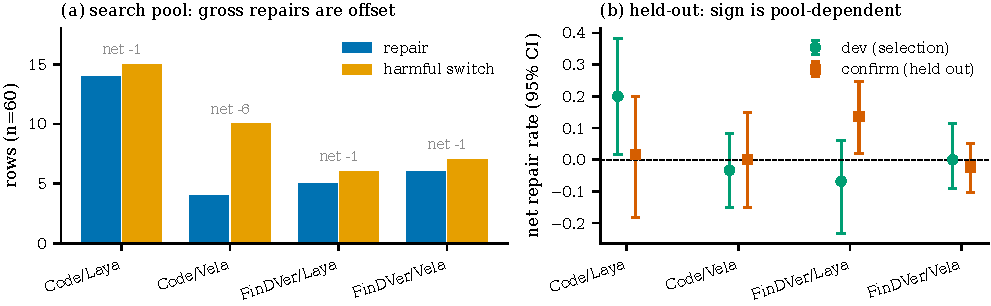
\includegraphics[width=0.92\linewidth]{../acl/figures/fig_headroom.pdf}
\caption{动作互补性。(a) 在训练池上，第二个动作修复错误，但也破坏正确答案；
每对柱上方印有净计数。(b) 同一 train 选出方向应用到 dev 与 confirm：净修复
的符号跨池变化，只有一个 confirm 单元的区间高于零。}
\label{fig:headroom}
\end{figure}

修复出现的位置与数量同样重要。把修复率对 \noul{} 概率分箱作图，
修复集中在中间与高带，约
$p\in[0.4,0.8]$，在最低带接近零。这与置信度级联的假设相反：阈值规则在
模型不确定时切换，而这恰恰是 \choice{} 最不可能修复任何东西的地方，因为
它能修复的行是 \noul{} 自信却错误的地方。这也解释了为什么校准救不了路由：
重校准单调地移动概率质量，但不会把可修复行从分布中部移到低置信度尾部。

第二个问题是 \choice{} 的有符号增量价值能否从第一次调用预测。表~\ref{tab:predictability}
使用 $\Delta_i=\mathbf{1}[\choice_i\text{ 正确}]-
\mathbf{1}[\noul_i\text{ 正确}]\in\{-1,0,+1\}$。所选模型的折外预测与真实
$\Delta$ 的 Spearman 相关为 $-0.02$、$+0.19$、$+0.13$ 和 $-0.17$；每个
分组自助法区间都包含零。有符号 $\Delta$ 的修复 AUROC 为 0.36、0.74、0.46
和 0.40，退化 AUROC 为 0.61、0.33、0.71 和 0.36。dev 选择的阈值（按成本
调整效用选择）给出的 confirm 原始净值为 $0.0$、$0.0$、$0.0$ 和 $-2.3$ 点，
成本调整净值为 $0.0$、$0.0$、$-0.1$ 和 $-2.8$ 点；没有单元为正，
FinDVer/Vela 的成本区间 $[-7.5,-0.1]$ 在负侧排除零。CodeXGLUE/Vela 选择
从不切换（0/60），因此两者都恰为零。始终切换基线为 $+1.7$、$0.0$、
$+13.6$ 和 $-2.3$，因此预测器放弃了 FinDVer/Laya 的全部 $+13.6$ 收益和
CodeXGLUE/Laya 的 $+1.7$ 收益。修复目标预测器达到更高的修复 AUROC
（最高 0.92），但同样在 confirm 上失败：排序修复不等于排序净效用。这里的
修复 AUROC 使用拟合的有符号 $\Delta$ 分数；下面的校准分析使用原始
\noul{} 概率，是另一个量。

\begin{table}[t]
\centering
\footnotesize
\caption{增量效用预测。折外 AUROC 在 \texttt{search\_train} 上使用分组感知
三折交叉验证；冠军模型与阈值在 \texttt{search\_dev} 上选择，冻结后用于
\texttt{confirm}。净效用为（修复 $-$ 退化）$/n$，单位为百分点，括号内为
计数；最后一列每次额外调用减去 $\lambda=0.05$。}
\label{tab:predictability}
\begin{tabular}{@{}lrrlrrr@{}}
\toprule
任务 / 模型 & LogReg 折外 & 树 折外 & 冠军 & dev 净 & confirm 净 & confirm 成本调整 \\
\midrule
CodeXGLUE / Laya & 0.674 & 0.739 & logreg & +20.0 (23/11) & +1.7 (17/16) & -3.3 \\
CodeXGLUE / Vela & 0.716 & 0.646 & logreg & +3.3 (7/5) & -1.7 (9/10) & -6.4 \\
FinDVer / Laya & 0.455 & 0.466 & tree & +1.7 (1/0) & +2.3 (1/0) & +1.5 \\
FinDVer / Vela & 0.919 & 0.794 & logreg & +3.4 (4/2) & -2.3 (0/1) & -2.6 \\
\bottomrule
\end{tabular}
\end{table}


校准是对基于概率的路由失败最自然的解释，因此它作为对照。原始概率在
confirm 上校准很差：ECE 从 0.090 到 0.290，Brier 从 0.218 到 0.287。在
\texttt{search\_train} 上拟合的温度缩放在三个单元降低 ECE（到
0.045--0.169）与 Brier；FinDVer/Vela 的 ECE 与 Brier 都略升。可达到的
band 类别不变，但选出的策略移动：原始概率给出的 confirm 净修复为
$-5.0$、$0.0$、$+2.3$ 与 $-2.3$ 点，温度缩放后为 $-1.7$、$+1.7$、$0.0$
与 $0.0$，与阈值选择噪声一致，而不是新信号。
原始 \noul{} 概率的修复 AUROC 直接说明了这一点：四个单元分别为 0.791、
0.444、0.336 与 0.095；
在后两个单元中，概率把可修复行排到随机水平\emph{之下}。当前答案的校准概率
不是替代动作价值的校准概率。

第三个问题是搜索能否把已有信号转化为可部署策略。表~\ref{tab:search} 总结
了比较。GA 对随机搜索是优化器价值最干净的检验：五个种子、四个任务—模型
单元与三个池，共 60 组配对 macro-F1 比较，没有任何一组的区间排除零。GA 对
固定仅切换有五个显著正单元，全部在 FinDVer/Vela 训练池，效应约为 $+0.12$；
在 dev 与 confirm 上，40 组比较没有一组显著。预注册的部署比较——train 选出
的 GA 对 confirm 上的固定仅切换——在每个种子级单元中都不显著。ES 对随机
搜索在全部 30 组比较中不显著；ES 对固定切换有三个显著训练单元与一个显著
confirm 单元（CodeXGLUE/Laya，种子 17，$+0.176$），这是唯一的 confirm 级
正结果，且未在种子上复现。NSGA-II 部署在五个 dev 单元与一个 confirm 单元
中显著差于固定基线，没有正单元。搜索问题没有任何稳定的留出信号供任何优化器
发现。

\begin{table}[t]
\centering
\small
\caption{预注册协议下的搜索比较。计数为排除零的配对分组自助法 95\% 区间数；
“正”表示演化策略胜过所述基线。GA 与 ES 行在三个池、五个种子上使用
macro-F1；NSGA-II 行在 12 个 dev 与 12 个 confirm 单元上使用准确率。}
\label{tab:search}
\begin{tabular}{@{}lrrl@{}}
\toprule
比较 & 正 & 负 & 解读 \\
\midrule
GA 对随机 & 0 & 0 & 无优势 (60) \\
GA 对固定 & 5 & 0 & 仅训练池 (60) \\
ES 对随机 & 0 & 0 & 无优势 (30) \\
ES 对固定 & 4 & 0 & 一个 confirm (30) \\
NSGA-II 对固定 & 0 & 6 & 5 dev, 1 confirm \\
\bottomrule
\end{tabular}
\end{table}


轨迹诊断解释了为什么更多搜索没有帮助。在 21 次记录的 GA/ES 运行中，有 15
次的最优适应度在第 0 代之后不再提高。中性变异率为 0.68--0.73，因此大多数
变异产生的候选训练分数完全相同。两个 CodeXGLUE 单元的 train--dev 秩相关为
$-0.56$ 与 $-0.51$，意味着在 train 上看起来更好的候选在 dev 上往往更差；
FinDVer 单元为 $+0.44$ 与 $+0.99$。把 CodeXGLUE/Vela 的预算从 24 提高到
48 并没有缩小差距：GA 在 48 的上限下只评估了 22、17 与 23 个唯一基因组，
而随机搜索用满了 48 个。搜索不只是调参不足，而是信息不足。

锁定测试是最后检查。每个单元使用 60 条官方 test 行，模板与 GA 基因组在
任何 test 调用前冻结；GA 对固定切换的 macro-F1 差为 $+0.008$
$[-0.148,+0.163]$（CodeXGLUE/Laya）、$0.000$ $[0.000,0.000]$
（CodeXGLUE/Vela）、$0.000$ $[-0.046,+0.045]$（FinDVer/Laya）与 $+0.243$
$[+0.138,+0.318]$（FinDVer/Vela）。最后一个增益来自更差的固定动作：固定
切换 macro-F1 为 0.413，固定 \noul{} 为 0.677，而 GA 基本停留在 \noul{}
（1.00--1.05 次调用/行），并未胜过 \noul{}（seed 17 为 $-0.021$
$[-0.081,0.000]$；seed 23/41 为 0）。没有任何 GA 基因组在任何单元上胜过
更好的固定动作。

边界检查问这些结论是否是某个池或任务的产物。迁移一致地没有帮助：32 个
源—目标乘划分单元中六个显著，且全部为负（两个对角线，四个非对角线）。
故障图确认 15 个合格单元中的 13 个在 dev、10 个在 confirm；稳定的高严重度
区域是 ProcessBench 的中置信度带，两个模型在同一批行上一起失败。

表~\ref{tab:processbench} 报告同一池上的选择性预测基线。全覆盖时选择性
准确率为 Laya 0.133、Vela 0.083；50\% 目标覆盖为 0.100/0.069，25\% 为
0.105/0.143；AURC 为 0.894/0.883。置信度不足以让弃权买到准确率。

\begin{table}[t]
\centering
\small
\caption{ProcessBench 在 confirm 上的选择性预测。各列为全覆盖、50\% 目标覆盖与
25\% 目标覆盖下的选择性准确率；括号内为实际 confirm 覆盖率。阈值在
\texttt{selection\_dev} 上选择并冻结。AURC 为风险—覆盖曲线下面积（越低越好）。}
\label{tab:processbench}
\begin{tabular}{@{}lrrrr@{}}
\toprule
模型 & 全覆盖 & 50\% 目标 & 25\% 目标 & AURC \\
\midrule
Laya & 0.133 (1.00) & 0.100 (0.50) & 0.105 (0.32) & 0.894 \\
Vela & 0.083 (1.00) & 0.069 (0.48) & 0.143 (0.23) & 0.883 \\
\bottomrule
\end{tabular}
\end{table}


综合来看，三个问题描述了一个在优化器被要求解决之前就已经失败的路由问题：
RQ1 发现总互补性但没有稳定的净互补性，RQ2 发现排序信号但没有可靠的策略
价值，RQ3 发现没有留出优势，因为地形平坦，而且训练排序在关键处不能预测
dev 排序。校准改进的是另一个量：模型可以为它回答的问题报告更好的概率，
却仍然无法说明另一个问题是否会被回答得更好。

实践含义是工作顺序的改变。在构建路由器之前，先测量动作集在留出组上是否
有净互补性，以及候选特征能否把可修复行排到随机水平之上。如果任一检查失败，
更强的优化器不会有用；如果两者都通过，就可以在匹配预算下运行优化器比较，
并使用预注册的 confirm 比较。

\section{结论}

结构化决策模型承诺：每次带类型判断所附的概率，可以决定何时值得购买第二次
判断。我们在冻结的 Laya 与 Vela 模型上，跨代码缺陷检测、金融主张核验与
数学推理错误定位的实验，并不支持这一承诺。对带策略的演化搜索相对更好的
固定动作或预算匹配的随机搜索没有产生优势，而失败在动作集、替代动作价值的
可预测性以及搜索地形三处都可见。

总互补性真实存在——逐行 oracle 最多提高 23.3 个准确率点——但修复被有害切换
抵消，净余额很小、依赖指标且跨池不稳定。修复集中在 \noul{} 概率的中高带，
而置信度级联在低概率处切换。校准与动作价值预测分离：温度缩放改善 ECE 与
Brier，却不能改变行的排序；在两个 FinDVer 单元中，概率把可修复行排到随机
水平之下。搜索地形平坦：大多数变异中性，大多数运行在第 0 代就停滞，因此
训练排序在关键处不能预测 dev 排序。

这些限制也是结果的一部分：池很小，\noul{} 模板未经过审计，只运行了两个开源
模型，锁定测试仅在冻结协议下运行一次。下一步是一个预测替代动作增量价值、并以留出净效用
评判的监督目标。代码、数据与分析脚本见
\url{https://anonymous.4open.science/r/codex-eacl-8E1E/}。


\bibliographystyle{../acl/acl_natbib}
\bibliography{../acl/references}

\appendix
\section{附录}
\label{app:models}

\textbf{模型与动作接口。} 表~\ref{tab:models} 总结本文讨论的三个结构化决策
模型。只有 Laya 与 Vela 在本地运行；Jev 定义商业参考点，本文不评测。

\begin{table}[t]
\centering
\small
\caption{本文讨论的三个结构化决策模型。只有 Laya 与 Vela 在本地运行；
Jev 定义商业参考点，本文不评测。}
\label{tab:models}
\begin{tabular}{@{}p{1.3cm}p{3.7cm}p{4.4cm}p{3.7cm}@{}}
\toprule
模型 & 接口 & 训练路线 & 本文角色 \\
\midrule
Jev & 一次调用返回带类型的 \textsc{Noul}、\textsc{Choice} 与 \textsc{Score} 决策及概率 & TypeSafe 称其为 RLCD 与适当评分目标；完整配方未公开 & RLCD / System One 家族的参考点；未运行 \\
Laya 0.4.16 & ModernBERT-large 编码器加决策头，约 4.21 亿参数；\textsc{Noul}、\textsc{Choice}、\textsc{Score} & 上游称配方为 RLCD，使用 log、spherical 与 ranked probability 分数 & 所有实验中使用的开放 RLCD 模型 \\
Vela 2.0 0.3B & 22 层 ModernBERT，768 隐藏维，8{,}192 token；\textsc{Noul}、\textsc{Choice}、\textsc{Score}、\textsc{Span}、\textsc{Set} & 从 Decision-1.0-Kai 的 Choice 路径初始化，任务特定损失与路由数据；未称 RLCD & 接口匹配、配方不同的对照模型 \\
\bottomrule
\end{tabular}
\end{table}


\label{app:native}

\textbf{原生单动作基线。} 表~\ref{tab:native} 报告两个原生动作在
\texttt{search\_dev} 池上的准确率与平均每次调用延迟。这些数字定义了每个
搜索策略所比较的固定策略。两种表示的每次调用成本相近，因此适应度函数使用
调用次数，而不是模型特定的延迟项。峰值常驻内存用于记录 CPU-only 执行包络。

\begin{table}[t]
\centering
\small
\caption{60 行选择池（\texttt{search\_dev}，种子 17）上的原生单动作基线。
延迟是本地 CPU 上每次调用的均值，仅用于说明两种表示成本大致相同；它不用于
适应度函数。}
\label{tab:native}
\begin{tabular}{@{}llrrrrrr@{}}
\toprule
任务 & 模型 & $n$ & \textsc{Noul} 准确率 & \textsc{Choice} 准确率 & \textsc{Noul} ms & \textsc{Choice} ms & 峰值 RSS (MB) \\
\midrule
CodeXGLUE & Laya & 60 & 0.450 & 0.650 & 2304 & 2239 & 2114 \\
CodeXGLUE & Vela & 60 & 0.633 & 0.667 & 2437 & 2341 & 1931 \\
FinDVer & Laya & 59 & 0.712 & 0.644 & 2768 & 2741 & 2117 \\
FinDVer & Vela & 59 & 0.458 & 0.458 & 2394 & 2263 & 1795 \\
ProcessBench & Laya & 60 & 0.100 & -- & 2616 & -- & 2124 \\
ProcessBench & Vela & 60 & 0.100 & -- & 1577 & -- & 1747 \\
\bottomrule
\end{tabular}
\end{table}


\label{app:extra}

\textbf{互补性总览。} 图~\ref{fig:headroom} 可视化表~\ref{tab:complementarity}
背后的总修复与净修复计数，包括把 train 选出的方向原样应用到 dev 与 confirm。

\begin{figure}[t]
\centering
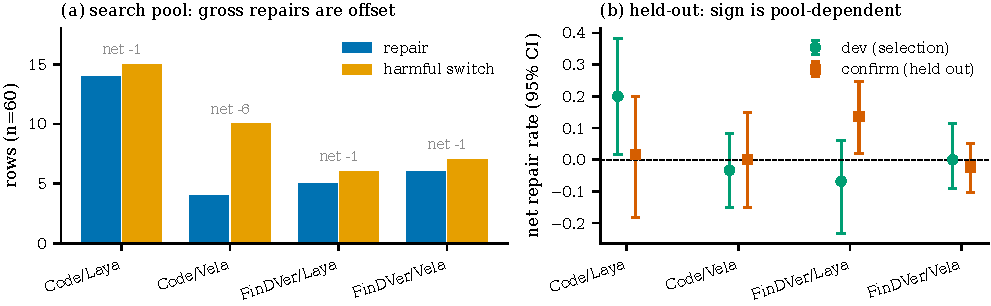
\includegraphics[width=0.96\linewidth]{../acl/figures/fig_headroom.pdf}
\caption{动作互补性。(a) 在训练池上，第二个动作修复错误，但也破坏正确答案；
每对柱上方印有净计数。(b) 同一 train 选出方向应用到 dev 与 confirm：净修复
的符号跨池变化，只有一个 confirm 单元的区间高于零。}
\label{fig:headroom}
\end{figure}

\textbf{修复轮廓。} 图~\ref{fig:repair} 显示第二个动作的修复率随 \noul{}
概率分箱的变化，分别给出训练、dev 与 confirm 池。每个点是该箱中 \noul{}
错误而 \choice{} 正确的行比例。当箱中至少有八行时印出箱计数。该图支持
第~\ref{sec:results} 节的论断：修复集中在概率中高段，而不是低置信度尾部。

\begin{figure}[t]
\centering
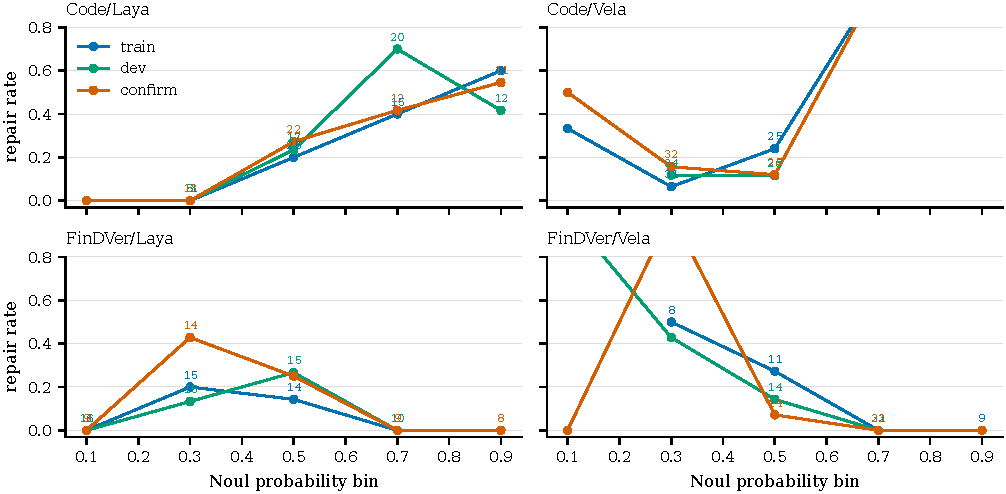
\includegraphics[width=0.96\linewidth]{../acl/figures/fig_repair_profile.pdf}
\caption{四个二元单元的修复率随 \noul{} 概率分箱的变化。最低箱中修复很少，
修复集中在 $p\in[0.4,0.8]$ 附近，而这正是置信度级联最不可能切换的地方。}
\label{fig:repair}
\end{figure}

\textbf{校准细节。} 表~\ref{tab:calibration} 报告校准及其与路由的关系；
图~\ref{fig:calibration} 画出四个二元单元在 confirm 上的可靠性图，包含温度
缩放前后。缩放参数在 \texttt{search\_train} 上拟合，原样应用到 confirm。
由于温度缩放是单调的，它改变数值概率，但不改变行的排序，因此也不改变路由
器可用的带策略集合。

\begin{table}[t]
\centering
\scriptsize
\setlength{\tabcolsep}{2.5pt}
\caption{\texttt{confirm} 上的校准及其与路由的关系。温度 $T$ 在
\texttt{search\_train} 上拟合；ECE 使用 15 个等宽箱。金标签 AUROC 是概率
排序当前动作正确性的能力；修复 AUROC 是它排序第二个动作可修复行的能力。
最后两列是在 \texttt{search\_dev} 上选择的带策略，分别用原始概率与温度
缩放概率得到的净修复。}
\label{tab:calibration}
\resizebox{\linewidth}{!}{%
\begin{tabular}{@{}lrrrrrrrr@{}}
\toprule
任务 / 模型 & ECE & ECE$_T$ & Brier & Brier$_T$ & AUROC$_{\text{金}}$ & AUROC$_{\text{修}}$ & 路由 & 路由$_T$ \\
\midrule
CodeXGLUE / Laya & 0.230 & 0.076 & 0.287 & 0.250 & 0.550 & 0.791 & -5.0 & -1.7 \\
CodeXGLUE / Vela & 0.090 & 0.045 & 0.260 & 0.250 & 0.522 & 0.444 & +0.0 & +1.7 \\
FinDVer / Laya & 0.290 & 0.141 & 0.285 & 0.246 & 0.603 & 0.336 & +2.3 & +0.0 \\
FinDVer / Vela & 0.147 & 0.169 & 0.218 & 0.234 & 0.605 & 0.095 & -2.3 & +0.0 \\
\bottomrule
\end{tabular}%
}
\end{table}


\begin{figure}[t]
\centering
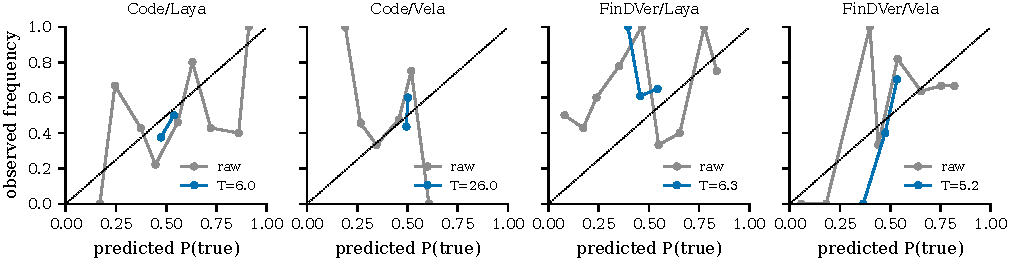
\includegraphics[width=0.96\linewidth]{../acl/figures/fig_calibration.pdf}
\caption{四个二元单元在 confirm 池上的可靠性图。灰色为原始 \noul{} 概率，
蓝色为温度缩放后。温度缩放降低校准误差，但它是单调映射：行的排序、以及
在重参数化意义下可用的带策略集合，都不变。}
\label{fig:calibration}
\end{figure}

\textbf{搜索诊断。} 图~\ref{fig:search} 汇总第~\ref{sec:results} 节讨论的
三个轨迹诊断：中性变异率、档案中训练与 dev 适应度的秩相关，以及种子 17 的
历史最优训练适应度。

\begin{figure}[t]
\centering
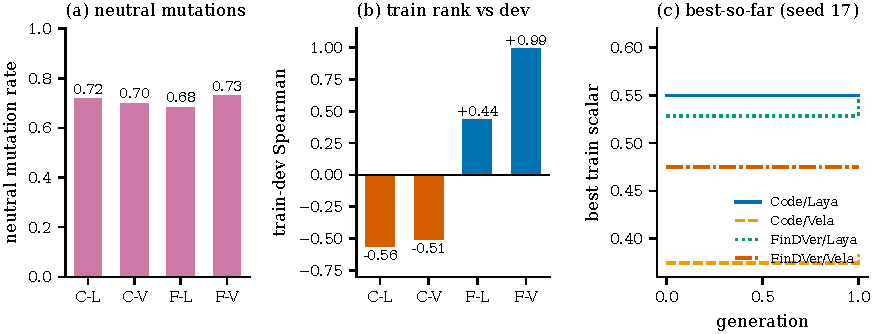
\includegraphics[width=0.96\linewidth]{../acl/figures/fig_search.pdf}
\caption{搜索诊断。(a) 68\% 到 73\% 的单基因变异不改变训练适应度。
(b) 档案中训练与 dev 适应度的秩相关在两个 CodeXGLUE 单元为负，在 FinDVer
为正。(c) 种子 17 的历史最优训练适应度；大多数运行最多改进一次，若干从
第 0 代起就平坦。}
\label{fig:search}
\end{figure}

\textbf{排序与策略价值。} 图~\ref{fig:predictability} 画出每个单元的折外
AUROC 与冻结的 dev 选择策略的 confirm 净效用。位于 0.5 右侧的点有排序信号；
位于零以下的点有负策略价值。分离清晰可见：排序信号最强的单元
（FinDVer/Vela）confirm 净值为负，而 confirm 净值最好的单元（FinDVer/Laya）
排序信号接近随机。

\begin{figure}[t]
\centering
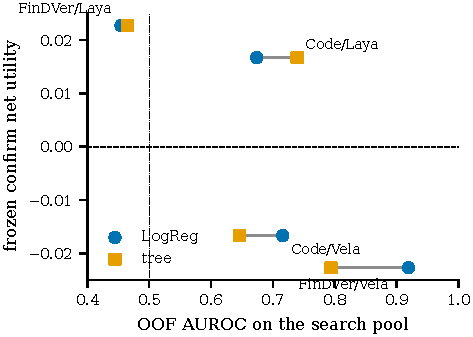
\includegraphics[width=0.78\linewidth]{../acl/figures/fig_predictability.pdf}
\caption{折外 AUROC 对 confirm 净效用。水平虚线为零净效用；垂直点线为随机
水平 AUROC。排序质量与策略价值不是同一个量。}
\label{fig:predictability}
\end{figure}

\label{app:boundary}

\textbf{边界检查。} 表~\ref{tab:boundary} 报告迁移计数与四个最高严重度的
故障图单元。图~\ref{fig:faultmap} 显示按任务、模型与置信带划分的完整
confirm 池严重度图。

\begin{table}[t]
\centering
\small
\caption{边界检查。上：冻结基因组迁移，统计相对目标固定仅切换策略的显著
配对准确率差异；对角线单元是同任务部署检查，非对角线单元是真正的迁移。
下：四个最高严重度的故障图单元，严重度定义为单元内错误率。}
\label{tab:boundary}
\begin{tabular}{@{}lrr@{}}
\toprule
迁移 & 显著正 & 显著负 \\
\midrule
对角线（同任务） & 0 & 2 \\
非对角线（真正迁移） & 0 & 4 \\
\bottomrule
\end{tabular}

\vspace{4pt}
\begin{tabular}{@{}lrrrrrr@{}}
\toprule
故障图单元 & $n$ discover & 严重度 & $n$ dev & 严重度 & $n$ confirm & 严重度 \\
\midrule
ProcessBench / Vela / 中 & 14 & 0.929 & 10 & 0.800 & 12 & 0.833 \\
ProcessBench / Laya / 中 & 13 & 0.923 & 15 & 0.867 & 16 & 0.875 \\
ProcessBench / Vela / 低 & 45 & 0.889 & 46 & 0.957 & 47 & 0.936 \\
ProcessBench / Laya / 高 & 41 & 0.756 & 35 & 0.914 & 38 & 0.895 \\
\bottomrule
\end{tabular}
\end{table}


\begin{figure}[t]
\centering
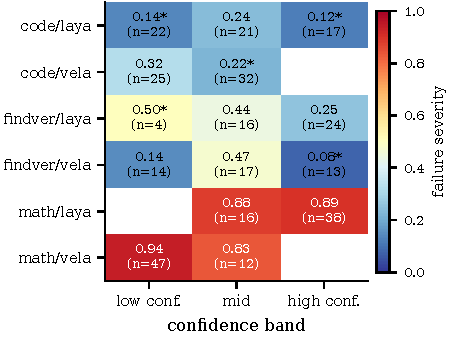
\includegraphics[width=0.78\linewidth]{../acl/figures/fig_faultmap.pdf}
\caption{按任务、模型与置信带划分的 confirm 池失败严重度。星号标记未在
0.15 容差内确认的单元。稳定的高严重度区域是 ProcessBench 的中置信度带，
两种表示在这里一起失败。}
\label{fig:faultmap}
\end{figure}

\textbf{复现细节。} 本文所有结果都来自已提交的 JSON 文件。逐行缓存是每个池
一个 JSON 文件，命名为 \texttt{cache\_<split>\_<task>\_<model>.json}，位于
\texttt{results/v4/evolution/} 下。分析脚本包括：
\begin{itemize}\setlength{\itemsep}{0pt}\setlength{\parskip}{0pt}
\item \texttt{scripts/analyze\_action\_complementarity.py}
\item \texttt{analyze\_complementarity\_heldout.py}
\item \texttt{analyze\_utility\_predictability.py}
\item \texttt{analyze\_search\_landscape.py}
\item \texttt{analyze\_transfer\_heldout.py}
\item \texttt{analyze\_calibration.py}
\item \texttt{analyze\_seed\_extension.py}
\item \texttt{analyze\_fixed\_action\_cis.py}
\item \texttt{analyze\_search\_dynamics.py}
\end{itemize}
表由 \texttt{scripts/make\_paper\_tables.py} 生成，图由
\texttt{scripts/plot\_paper\_figures.py} 生成；两个脚本都不含手抄数字。
GA/ES/NSGA-II 运行器位于 \texttt{src/evolution/}。模型修订、数据集修订、
种子与 CPU 线程数记录在每个结果文件的元数据中。五种子扩展使用种子 17、23、
41、59 与 73；预算探针使用同一缓存，唯一基因组上限为 48。不使用托管 CI
运行器：每次模型调用都在本地 Windows 机器上执行，缓存输出是本文分析的唯一
输入。

\textbf{未报告的内容。} 锁定测试未运行，\noul{} 模板未针对替代措辞审计，
没有为每个搜索策略测量真实端到端延迟，Jev 未评测。这些省略在正文中说明，
没有用代理数字填补。FinDVer/Laya confirm 单元是唯一净修复准确率区间为正的
单元；应把它视为更大规模复现的线索，而不是可部署结果。


\end{document}
